\protect\hyperlink{main-nav}{≡} \protect\hyperlink{close-nav}{×}

\hypertarget{section-1.5-quadratics}{%
\section{Section 1.5: Quadratics}\label{section-1.5-quadratics}}

Quadratics are transformations of the function \textbackslash{}(
f(x)=x\^{}2 \textbackslash{}). Quadratics commonly arise from problems
involving area and projectile motion, providing some interesting
applications.

\hypertarget{example-1}{%
\paragraph{Example 1}\label{example-1}}

A backyard farmer wants to enclose a rectangular space for a new garden.
She has purchased 80 feet of wire fencing to enclose three sides, and
will put the fourth side against the backyard fence. Find a formula for
the area enclosed by the fence if the sides of fencing perpendicular to
the existing fence have length \textbackslash{}(L\textbackslash{}).

In a scenario like this involving geometry, it is often helpful to draw
a picture. It might also be helpful to introduce a temporary variable,
\textbackslash{}(W\textbackslash{}), to represent the side of fencing
parallel to the fourth side or backyard fence.

\begin{figure}
\centering
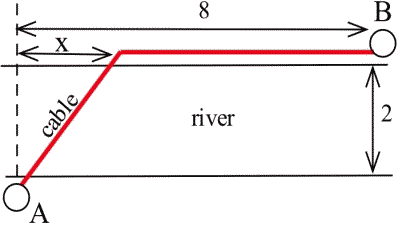
\includegraphics{images/image096.png}
\caption{}
\end{figure}

Since we know we only have 80 feet of fence available, we know that
\textbackslash{}( L+W+L=80 \textbackslash{}), or more simply,
\textbackslash{}( 2L+W=80 \textbackslash{}). This allows us to represent
the width, \textbackslash{}(W\textbackslash{}), in terms of
\textbackslash{}(L\textbackslash{}): \textbackslash{}( W=80-2L
\textbackslash{})

Now we are ready to write an equation for the area the fence encloses.
We know the area of a rectangle is length multiplied by width, so
\textbackslash{}( A=LW=L(80-2l) \textbackslash{}), so
\textbackslash{}{[} A(L)=80L-2L\^{}2. \textbackslash{}{]} This formula
represents the area of the fence in terms of the variable length
\textbackslash{}(L\textbackslash{}).

\hypertarget{forms-of-quadratic-functions}{%
\paragraph{Forms of Quadratic
Functions}\label{forms-of-quadratic-functions}}

The \textbf{standard form} of a quadratic function is \textbackslash{}(
f(x)=ax\^{}2+bx+c \textbackslash{}).

The \textbf{transformation form} of a quadratic function is
\textbackslash{}( f(x)=a(x-h)\^{}2+k \textbackslash{}).

The \textbf{vertex} of the quadratic function is located at
\textbackslash{}((h, k)\textbackslash{}), where
\textbackslash{}(h\textbackslash{}) and
\textbackslash{}(k\textbackslash{}) are the numbers in the
transformation form of the function. Because the vertex appears in the
transformation form, it is often called the \textbf{vertex form}.

\hypertarget{example-2}{%
\paragraph{Example 2}\label{example-2}}

Write an equation for the quadratic graphed below as a transformation of
\textbackslash{}( f(x)=x\^{}2 \textbackslash{}).

\begin{figure}
\centering
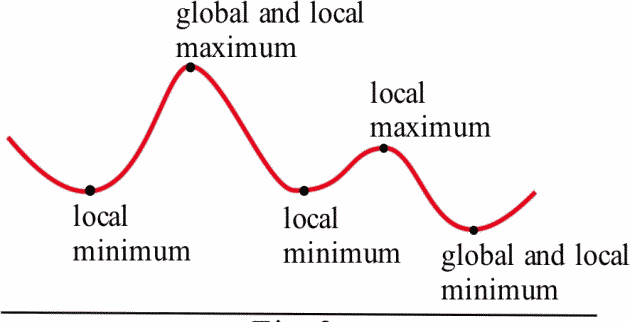
\includegraphics{images/image057.png}
\caption{}
\end{figure}

We can see the graph is the basic quadratic shifted to the left 2 and
down 3, putting the vertex at \textbackslash{}((-2,
-3)\textbackslash{}), giving a formula in the form \textbackslash{}(
g(x)=a(x+2)\^{}2-3 \textbackslash{}). By plugging in a point that falls
on the grid, such as \textbackslash{}((0,-1)\textbackslash{}), we can
solve for the stretch factor:
\textbackslash{}{[}\textbackslash{}begin\{align*\} -1=\&a(0+2)\^{}2-3
\textbackslash{}\textbackslash{} 2=\& 4a
\textbackslash{}\textbackslash{} a=\& \textbackslash{}frac\{1\}\{2\}
\textbackslash{}end\{align*\}\textbackslash{}{]}

The equation for this formula is \textbackslash{}{[}
g(x)=\textbackslash{}frac\{1\}\{2\}(x+2)\^{}2-3 \textbackslash{}{]}

To view this video please enable JavaScript, and consider upgrading to a
web browser that \href{http://videojs.com/html5-video-support/}{supports
HTML5 video}

\hypertarget{short-run-behavior-intercepts}{%
\subsubsection{Short run Behavior:
Intercepts}\label{short-run-behavior-intercepts}}

As with any function, we can find the vertical intercepts of a quadratic
by evaluating the function at an input of zero, and we can find the
horizontal intercepts by solving for when the output will be zero.
Notice that depending upon the location of the graph, we might have
zero, one, or two horizontal intercepts.

\begin{figure}
\centering
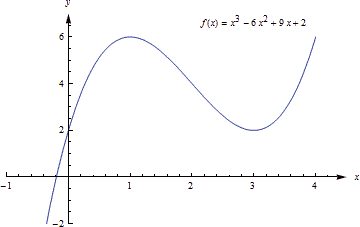
\includegraphics{images/image058.png}
\caption{Zero horizontal intercepts}
\end{figure}

\begin{figure}
\centering
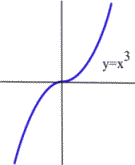
\includegraphics{images/image059.png}
\caption{One horizontal intercept}
\end{figure}

\begin{figure}
\centering
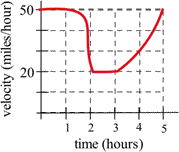
\includegraphics{images/image060.png}
\caption{Two horizontal intercepts}
\end{figure}

Notice that in the standard form of a quadratic, the constant term c
reveals the vertical intercept of the graph, since \textbackslash{}(
f(0)=a(0)\^{}2+b(0)+c=c \textbackslash{}).

\hypertarget{example-3}{%
\paragraph{Example 3}\label{example-3}}

Find the vertical and horizontal intercepts of the quadratic
\textbackslash{}( f(x)=3x\^{}2+5x-2 \textbackslash{}).

We can find the vertical intercept by evaluating the function at an
input of zero:
\textbackslash{}{[}f(0)=3(0)\^{}2+5(0)-2=-2\textbackslash{}{]} So the
vertical intercept is at (0,-2)

For the horizontal intercepts, we solve for when the output will be
zero: \textbackslash{}{[}0=3x\^{}2+5x-2.\textbackslash{}{]} In this
case, the quadratic can be factored easily, providing the simplest
method for solution.:
\textbackslash{}{[}0=(3x-1)(x+2),\textbackslash{}{]} so either
\textbackslash{}{[} \textbackslash{}begin\{align*\} 0=\&
3x-1\textbackslash{}\textbackslash{} x=\& \textbackslash{}frac\{1\}\{3\}
\textbackslash{}end\{align*\} \textbackslash{}{]} or \textbackslash{}{[}
\textbackslash{}begin\{align*\} 0=\& x+2\textbackslash{}\textbackslash{}
x=\& -2 \textbackslash{}end\{align*\} \textbackslash{}{]} So the
Horizontal intercepts are at \textbackslash{}(
\textbackslash{}left(\textbackslash{}frac\{1\}\{3\},0\textbackslash{}right)
\textbackslash{}) and \textbackslash{}((-2,0)\textbackslash{}).

When a quadratic is not factorable or is hard to factor, we can turn to
the quadratic formula.

\hypertarget{quadratic-formula}{%
\paragraph{Quadratic Formula}\label{quadratic-formula}}

For a quadratic function given in standard form \textbackslash{}(
f(x)=ax\^{}2+bx+c \textbackslash{}), the \textbf{quadratic formula}
gives the horizontal intercepts of the graph of this
function:\textbackslash{}{[}
x=\textbackslash{}frac\{-b\textbackslash{}pm
\textbackslash{}sqrt\{b\^{}2-4ac\}\}\{2a\} \textbackslash{}{]}

To view this video please enable JavaScript, and consider upgrading to a
web browser that \href{http://videojs.com/html5-video-support/}{supports
HTML5 video}

\hypertarget{example-4}{%
\paragraph{Example 4}\label{example-4}}

A ball is thrown upwards from the top of a 40 foot high building at a
speed of 80 feet per second. The ball's height above ground can be
modeled by the equation \textbackslash{}{[} H(t)=-16t\^{}2+80t+40
.\textbackslash{}{]} When does the ball hit the ground?

To find when the ball hits the ground, we need to determine when the
height is zero, i.e., when \textbackslash{}(H(t) = 0\textbackslash{}).
While we could do this using the transformation form of the quadratic,
we can also use the quadratic formula: \textbackslash{}{[}
t=\textbackslash{}frac\{-80\textbackslash{}pm
\textbackslash{}sqrt\{80\^{}2-4(-16)(40)\}\}\{2(-16)\}=\textbackslash{}frac\{-80\textbackslash{}pm\textbackslash{}sqrt\{8960\}\}\{-32\}
\textbackslash{}{]}

Since the square root does not simplify nicely, we can use a calculator
to approximate the values of the solutions:\textbackslash{}{[}
t=\textbackslash{}frac\{-80-\textbackslash{}sqrt\{8960\}\}\{-32\}\textbackslash{}approx
5.458 \textbackslash{}quad\textbackslash{}text\{or\}\textbackslash{}quad
t=\textbackslash{}frac\{-80+\textbackslash{}sqrt\{8960\}\}\{-32\}\textbackslash{}approx
-0.458 \textbackslash{}{]}

The second answer is outside the reasonable domain of our model, so we
conclude the ball will hit the ground after about 5.458 seconds.

\begin{longtable}[]{@{}ll@{}}
\toprule
\endhead
\href{section1-4.php}{← Previous Section} & \href{section1-6.php}{Next
Section →}\tabularnewline
\bottomrule
\end{longtable}
